% demo.tex
%
% Enjoy, evolve, and share!
%
% Compile it as follows:
%   latexmk
%
% Check file `dithesis.cls' for other configuration options.
%
\documentclass[inscr,ack,preface]{dithesis}

%\usepackage{graphicx}

%%%%%%%%%%%%%%%%%%%%%%%%%%%%%%%%%%%%%%%%%%%%%%%%%%%%%%%%%%%%%%%%%%%%%%%%%%%%%%%
%%%%%%%%%%%%%%%%%%%% User-specific package inclusions %%%%%%%%%%%%%%%%%%%%%%%%%
%%%%%%%%%%%%%%%%%%%%%%%%%%%%%%%%%%%%%%%%%%%%%%%%%%%%%%%%%%%%%%%%%%%%%%%%%%%%%%%
\usepackage{booktabs}
\usepackage{hyperref}
\usepackage{lipsum}
\usepackage{enumerate}
\usepackage{amsmath}
\usepackage{amssymb}
\usepackage{listings}

\hypersetup{
    unicode=true,                     % non-Latin characters in bookmarks
    pdffitwindow=true,                % page fit to window when opened
    pdfnewwindow=true,                % links in new window
    pdfkeywords={},                   % list of keywords
    colorlinks=true,                  % false: boxed links; true: colored links
    linkcolor=black,                  % color of internal links
    citecolor=black,                  % color of links to bibliography
    filecolor=black,                  % color of file links
    urlcolor=black,                   % color of external links
    pdftitle={},                      % title
    pdfauthor={},                     % author
    pdfsubject={}                     % subject of the document
}
%%%%%%%%%%%%%%%%%%%%%%%%%%%%%%%%%%%%%%%%%%%%%%%%%%%%%%%%%%%%%%%%%%%%%%%%%%%%%%%
%%%%%%%%%%%%%%%%%%%% User-specific package inclusions %%%%%%%%%%%%%%%%%%%%%%%%%
%%%%%%%%%%%%%%%%%%%%%%%%%%%%%%%%%%%%%%%%%%%%%%%%%%%%%%%%%%%%%%%%%%%%%%%%%%%%%%%


%%%%%%%%%%%%%%%%%%%%%%%%%%%%%%%%%%%%%%%%%%%%%%%%%%%%%%%%%%%%%%%%%%%%%%%%%%%%%%%
%%%%%%%%%%%%%%%%%%%%%% User-specific configuration %%%%%%%%%%%%%%%%%%%%%%%%%%%%
%%%%%%%%%%%%%%%%%%%%%%%%%%%%%%%%%%%%%%%%%%%%%%%%%%%%%%%%%%%%%%%%%%%%%%%%%%%%%%%
%%%%%%%%%%%%%%%%%%%%%%%%%%%%%%%%%%%%%%%%%%%%%%%%%%%%%%%%%%%%%%%%%%%%%%%%%%%%%%%
%%%%%%%%%%%%%%%%%%%%%% User-specific configuration %%%%%%%%%%%%%%%%%%%%%%%%%%%%
%%%%%%%%%%%%%%%%%%%%%%%%%%%%%%%%%%%%%%%%%%%%%%%%%%%%%%%%%%%%%%%%%%%%%%%%%%%%%%%


%%%%%%%%%%%%%%%%%%%%%%%%%%%%%%%%%%%%%%%%%%%%%%%%%%%%%%%%%%%%%%%%%%%%%%%%%%%%%%%
%%%%%%%%%%%%%%%%%%%%%%%%%%% Required Metadata %%%%%%%%%%%%%%%%%%%%%%%%%%%%%%%%%
%%%%%%%%%%%%%%%%%%%%%%%%%%%%%%%%%%%%%%%%%%%%%%%%%%%%%%%%%%%%%%%%%%%%%%%%%%%%%%%
%
% First name, last name
%
\authorFirstGr{Νικόλαος}
\authorFirstAbrGr{Ν.} % abbreviation of first name
\authorMiddleGr{Γ.}   % abbreviation of father's first name
\authorLastGr{Γαλάνης}
\authorFirstEn{Nikolaos}
\authorFirstAbrEn{N.}
\authorMiddleEn{G.}
\authorLastEn{Galanis}
\authorSn{1115201700019}

%
% The title of the thesis
%
\titleEn{Real World Applications of Differential Data Privacy}
\titleGr{Εφαρμογές της Διαφορικής Ιδιωτικότητας Δεδομένων}

%
% Month followed by Year
%
\dateGr{ΙΟΥΝΙΟΣ 2021}
\dateEn{JUNE 2021}

%
% Supervisor(s) info
%
\supervisorGr{Κωνσταντίνος Χατζηκοκολάκης}{Αναπληρωτής Καθηγητής}
\supervisorEn{Konstantinos Chatzikokolakis}{Associate Professor}

%
% Abstract, synopsis, inscription, ack, and preface pages.
%
% \setlength\parindent{24pt}

\abstractEn{
\par The problem of preserving privacy while extracting information during data analysis, has been an everlasting one. Specifically, during the big-data era, user details can be easily compromised by a malicious handler, something considered both as a security, and as a privacy issue.
\par With that being the case, there is a simple solution of denying the access to user data, thus making the mining of useful information about a plethora of subjects impossible. On the other hand, a successful mechanism would be for the data to be flowing without control, something that would be beneficiary for the advance of sciences (because of the huge amount of information that would be available), but a significant compromisation for the individuals' privacy. \par
However, none of these two solutions are applicable and helpful for solving our problem. The answer is finding a balance, that would benefit both parties: the users and their privacy, as well as the researchers. The optimal fix to the subject, is Differential Privacy, which is actually a promise, made by the data handler to the user, that they will not be affected, by allowing their data to be used in any analysis, no matter what other studies/databases/info resources are available. Meanwhile, the output data statistics should be accurate enough for any researcher to extract useful information from them.\par
This is a promise that in the first sight, seems rather hard to be achieved. Despite that, during this thesis, we will look closely into the theory which makes this form of privacy possible, by the addition of random noise to the user data. Differential Privacy is based on probabilistic theories, well known from the $20^{th}$ century, however, it is a rather new technique, which has yet to be fully implemented in a handy way for all data-miners to use.
\par The goal of this thesis, is to examine and compare previously created mechanisms for D.P., while also creating our own mechanism, that serves to the purpose of achieving Local D.P., a form of Differential Privacy that is nowadays widely used in machine learning algorithms, aiming to protect the individuals that send their personal data for analysis. We will do so, by creating a library that is easy to use, and applies to all the rules of data privacy, and then extract conclusions from its use.
}
\abstractGr{
Το πρόβλημα της διατήρησης της ιδιωτικότητας κατά την ανάλυση δεδομένων, υφίσταται για πολύ καιρό. Συγκεκριμένα, στην εποχή των big-data, λεπτομέρειες των χρηστών μπορούν εύκολα να παραβιαστούν από κακόβουλους χειριστές των δεδομένων, γεγονός που θεωρείται ζήτημα τόσο όσον αφορά την ασφάλεια, όσο και την προστασία της ιδιωτικότητας του ατόμου.\par
Mε την υπάρχουσα κατάσταση, υπάρχει η απλή λύση της άρνησης της πρόσβασης σε δεδομένα χρηστών, στον βωμό της προστασίας τους, κάτι που καθιστά την εξαγωγή συμπερασμάτων για ποικίλα θέματα αδύνατη. Από την άλλη, ένας επιτυχημένος μηχανισμός θα ήταν η ελεύθερη διακίνηση των δεδομένων, χωρίς φιλτράρισμά τους, γεγονός που θα ήταν ωφέλιμο για την πρόοδο των επιστημών (λόγω του μεγάλου όγκου δεδομένων που θα ήταν διαθέσιμος), αλλά μία μεγάλη παραβίαση της ιδιωτικότητας των ατόμων. 
\par 
Ωστόσο, καμία από τις δύο αυτές λύσεις δεν μπορεί να εφαρμοστεί και να μας βοηθήσει στην επίλυση τους προβλήματός μας. Η απάντηση είναι η εύρεση μίας ισορροπίας, η οποία ευνοεί και τα δύο μέρη: τους χρήστες και την ιδιωτικότητά τους, όπως και τους ερευνητές. Η βέλτιστη επίλυση του θέματος, είναι η Διαφορική Ιδιωτικότητα, που στην πραγματικότητα πρόκειται για μία υπόσχεση από τον χειριστή των δεδομένων προς τον χρήστη, πως ο χρήστης δεν θα επηρεαστεί αν επιτρέψει τη χρήση των δεδομένων του σε κάποια ανάλυση, χωρίς περιορισμούς όπως η παράλληλη ύπαρξη άλλων μελετών/βάσεων δεδομένων/πληροφοριών που υπάρχουν για αυτόν. Παράλληλα, τα στατιστικά του αποτελέσματος της ανάλυσης, πρέπει να είναι αρκετά ακριβή, ώστε ο ερευνητής να μπορεί να εξάγει χρήσιμη πληροφορία από αυτά. \par 
Η υπόσχεση αυτή, δείχνει δύσκολα υλοποιήσιμη με την πρώτη ματιά. Παρόλα αυτά, σε αυτήν την πτυχιακή εργασία, θα ερευνήσουμε με λεπτομέρεια τη θεωρία που καθιστά εφικτή αυτή τη μορφή ιδιωτικότητας, με την προσθήκη τυχαίου θορύβου στα δεδομένα. Η Διαφορική Ιδιωτικότητα βασίζεται σε πιθανοτικές κατανομές, γνωστές ήδη από τον $20^o$ αιώνα, όμως παραμένει μία νέα τεχνική, η οποία δεν έχει πλήρως υλοποιηθεί με τρόπο τέτοιον ώστε να μπορεί να χρησιμοποιηθεί από πολλούς ανθρώπους που είναι υπεύθυνοι για την εξαγωγή δεδομένων.
\par Σκοπός αυτής της πτυχιακής εργασίας, είναι να μελετήσουμε και να συγκρίνουμε ήδη υλοποιημένους μηχανισμούς πανω στην Δ.Ι., ενώ παράλληλα θα δημιουργήσουμε τον δικό μας μηχανισμό, ο οποίος χρησιμοποιείται για τους σκοπούς της Τοπικής Διαφορικής Ιδιωτικότητας που συναντάται την σήμερον ημέραν σε αλγορίθμους μηχανικής μάθησης, με στόχο να προστατέψει τα δεδομένα που αποστέλλουν για εκμάθηση οι χρήστες. Θα το κατορθώσουμε αυτό δημιουργώντας μία προγραμματιστική βιβλιοθήκη η οποία είναι εύκολη στη χρήση, ικανοποιώνατας παράλληλα τους κανόνες της προστασίας δεδομένων, και τέλος θα εξάγουμε συμπεράσματα από τη χρήση της βιβλιοθήκης αυτής.

}
\acksEn{
\begin{greek}
Στη σελίδα αυτή αναφέρονται οι ευχαριστίες. Η σελίδα αυτή είναι προαιρετική. Παρατίθεται παράδειγμα ευχαριστιών.

Για τη διεκπεραίωση της παρούσας Πτυχιακής Εργασίας, θα θέλαμε να ευχαριστήσουμε τους επιβλέποντες, αν. καθ .Ευστράτιο Γεωργιάδη, Γρηγόριο Παπάμαλο, Αναστασία Γούσιου, Ξενοφών Παπαδόπουλο, για τη συνεργασία και την πολύτιμη συμβολή του στην ολοκλήρωση της.
\end{greek}
}
\prefaceEn{
\begin{greek}
Στον πρόλογο αναφέρονται θέματα που δεν είναι επιστημονικά ή τεχνικά, όπως το πλαίσιο που διενεργήθηκε η εργασία, ευχαριστίες, ο τόπος διεξαγωγής κλπ.
\end{greek}
}

\inscriptionEn{\emph{Στη σελίδα αυτή αναφέρονται οι αφιερώσεις. Η σελίδα αυτή είναι προαιρετική.}}

%
% Subject area and keywords
%
\subjectAreaGr{Προστασία και Ιδιωτικότητα Δεδομένων}
\subjectAreaEn{Data Privacy}
\keywordsGr{Διαφορική Ιδιωτικότητα, Ασφάλεια, Δεδομένα Χρηστών, Προστασία Δεδομένων, Θόρυβος σε Δεδομένα, Συλλογή Δεδομένων}
\keywordsEn{Differential Privacy, Security, User data, Data Privacy, Noisy Data, Aggregation of Data}

%
% Set the .bib file containing your paper publications (leave the extension out)
%
% This is optional, but it should be specified when option 'lop' is passed to
% the document class.
%
% Then, inside the document environment, you may use the command '\nocitelop' to
% site your papers, as you would traditionally do with the commands '\cite' or
% '\nocite'.
%
% The papers are printed in reverse chronological order.
%
%\lopfile{mypapers/pubs}
%%%%%%%%%%%%%%%%%%%%%%%%%%%%%%%%%%%%%%%%%%%%%%%%%%%%%%%%%%%%%%%%%%%%%%%%%%%%%%%
%%%%%%%%%%%%%%%%%%%%%%%%%%% Required Metadata %%%%%%%%%%%%%%%%%%%%%%%%%%%%%%%%%
%%%%%%%%%%%%%%%%%%%%%%%%%%%%%%%%%%%%%%%%%%%%%%%%%%%%%%%%%%%%%%%%%%%%%%%%%%%%%%%

\begin{document}

\frontmatter

\mainmatter

\chapter{INTRODUCTION}

\section{Need for Privacy}


\par In our days, data is everywhere, including our smartphones, our computers our TVs, even our watches. Every device and nearly every website track down data, in order to provide more personalized services. This, of course, is desired by the users, as they are more likely to see relevant advertisements, and in general, have a more unique experience while they are using their devices.

\par At the same time, the services that track down the data are also benefited, because of the way that science evolves: Experiments need to be made, thus the more available data in order to conduct them, the better. As an example, we might think the medical community: when someone logs-in to the hospital, it is beneficiary for the doctors to gather his data, in order to study his decease, and his potential recovery, not only for the shake of the patient, but also for the further study of the decease. 

\par While providing data may seem inevitable and yet beneficiary for all parties, there is always a risk that this data will be used in order to compromise the user's privacy. When the information lands in the wrong hands, it can expose some characteristics of the user that he does not want to be shared. In our medical example, let's now consider a patient with a rare decease, who logs-in to a local hospital. He might consent to share his personal data (name, age etc.), but only for the doctors to use it. What will happen when the doctors give the data of the whole hospital for analysis? This patient, considering he is one of the few that has this illness, may be stigmatized,  when the data analysts find out his condition. Wouldn't it be better for him, if, let's say, his name was not exposed? We will see later on, why this approach, is found to be successful, but not enough, for extreme cases.

\section{Definition of the problem of privacy}
\par In general, when we consider the \textbf{problem of privacy}, we refer to the protection of the disclosure of sensitive information of individuals, when a collection of data about these individuals (dataset) is made publicly available.

\subsection{Achieving Privacy via Anonymization}

\par One of the first, and rather successful attempts for preserving privacy, was anonymization, meaning removing all personal identifiers from the dataset. This technique is further developed, using famous algorithms like k-anonymity, l-diversity etc. However, there are several problems with this approach. Firstly, they are very computational heavy, as their complexity rises up to an exponential one, making the anonymization of a large dataset very slow. Also, the anonymization does not guarantee that the user will remain private, if other datasets are not anonymized. Let's once again consider our example. Suppose our patient goes to two separate hospitals for his treatment, and one of them uses the best anonymization techniques, while the other one provides the data without any form of privacy. Our patient is on both of the datasets, thus the techniques adopted by the first hospital are now useless. This expands to the real world, because, no matter how careful you (and the services that you use) are, a single data breach is enough for you to be compromised. 

\par So, right now, things seem a bit pessimistic, supposing that anonymization, no matter how well performed, can not fix our problem. Another successful technique, that is used on many fields, is the addition of noise. During a later section, we are going to examine in which ways it can benefit us while trying to solve our problem.

\subsection{Achieving Privacy via Randomization}

Randomization can be applied to the data of the users in two different forms:
\begin{itemize}
    \item Apply random noise \textbf{directly to the data}. This will result to altered data, which will then be processed, so that the adversary will not be able to individualize the entries in the dataset.
    \item Apply random noise to \textbf{queries asked to the dataset}. In that case, the dataset is not directly available to the analysts. Instead, they are allowed to ask questions to the dataset, and the answers are then being randomized, and returned.
\end{itemize}

Both the above approaches are utilized, but the second one is widely preferred. During our analysis of data privacy, we are going to dive in both of those techniques, as well as the libraries that they are used in.

\par As we can see, the randomization method looks good in theory, but we must answer to several questions before implementing it, such as:

\begin{itemize}
    \item How can we define privacy for noisy queries?
    \item What type of noise do we need?
    \item What should we do in the case of extreme amount of noise added?
\end{itemize}

We are going to answer those questions later on, during our next chapters. 

\section{Goal of this thesis}
As discussed in the introduction, that the most effective up-to date method for applying privacy into a dataset, is via randomization. The method used, is called \textbf{Differential Privacy}, and is based on injecting noise into the users' data. 

The theory behind this method includes many mathematical theorems, however, it can by easily explained. We will proceed by taking a look on those principles, and analysing the theory behind this form on data privacy. Then, we will proceed by examining some existing applications of D.P., especially some libraries that help us to apply this technique in a dataset. Finally, we are going to create our own library in order to apply Local D.P., a form of privacy that we will discuss in the next chapter. 

This library will allow a user to fully anonymize a dataset, and afterwards create histogram and counting queries for this dataset. During the implementation of this library, a new protocol will be introduced, which follows the rules of D.P., and produces better results than many already-existing protocols.


\chapter{PRINCIPLES OF DIFFERENTIAL PRIVACY}

During this chapter we are going to introduce the term of D.P., and its definition, alongside with the principles that need to be followed while applying it.

\section{Promise of Differential Privacy}

\par Differential Privacy is actually a promise made by the data handlers, to the participants of a study: "You will not be affected, adversely or otherwise, by allowing your data to be used in any study or analysis, no matter what other studies/ datasets/ info resources are available". 
\par The goal is to make the data widely available for analysis, while protecting the users. However, is it possible to learn nothing about an individual, while gathering useful information about a population? This is actually what D.P. is trying to achieve.


\section{Definition of Differential Privacy}
Before defining D.P., we must analyze some of the basic components of its definition.

\subsection{Randomized Response}
Randomized response is one of the earliest privacy mechanisms, that is used to conduct surveys where taboo behaviour is studied. The participants in those surveys are asked to answer truthfully, while they do not want to be stigmatized. There is a micro-world of what we are trying to achieve, thus we are going to give the algorithm of the randomized response in order to answer a binary (yes/no) question.

\begin{itemize}
    \item Flip a coin.
    \item If it lands on heads, answer truthfully
    \item If it lands on tails, flip another one
    \item If it lands on heads, answer no, else, answer yes
\end{itemize}

We are going to analyze this algorithm and its success in later chapters, but for now, it is enough to know that there exists a simple mechanism that adds noise, and is rather accurate for large samples.

Before giving the definition of D.P., we must define its components. 

\begin{itemize}
    \item \textbf{Probability Simplex}, given a discrete set $B$, is denoted as $\Delta(B)$ and is defined to be:
    \begin{align*}
        \Delta(B) = \{ x\in R^{|B|}: x_i \geq 0 \text { } \forall i \text{ and } \sum_{i=1}^{|B|} x_i = 1\}
    \end{align*}
    \item A \textbf {Randomized algorithm} $M$ with domain $A$ and discrete range of results $B$, is associated with the mapping $M: A\rightarrow\Delta(B)$. On
    \item \textbf{Distance between Databases:} The $l_1$ norm of a database x is denoted $||x||_1$ and it is defined to be: $||x||_1 = \sum_{i = 1}^{|x|} |x_i|$. Thus, the $l_1$ distance between 2 databases $x$ and $y$, is $||x-y||_1$, and the size of a database $x$ os $||x||_1$.
    
\end{itemize}
There are plenty definitions for D.P., but throughout this thesis we are going to use the one bellow.

\subsection{Definition}
Differential Privacy is defined as following:
\\
\\
A randomized algorithm $M$ with domain $N^{|x|}$ is (ε,δ)-differentially private, if for all $S \in Range(n)$ and for all $x,y \in N^{|x|}$ s.t. $||x - y||_1 \leq 1$
$$ Pr[M(x) \in S] \leq e^\epsilon Pr[M(y) \in S] + \delta$$

where the probability space is over the coin flips of the mechanisms $M$. If $\delta = 0$, we say that $M$ is ε-differentially private.

\\
It should be noted that D.P. is rather a definition than a strict algorithm. While relying on the definition of D.P., we can create different algorithms, which will all ensure that the result will be deferentially private. This allows us to create different forms of D.P., that will be analyzed later on this thesis.

The whole point of Differential Privacy, is that the output of a D.P. mechanism, should by \textbf{independent} of whether or not an individual is present in the domain $N$. The "ability" of the adversary to recognise the existence of a column in the dataset, is regularized by epsilon.

\section{The meaning of epsilon}
It is made clear from the above definition, that if we have a computational task, we might find different algorithms for applying D.P., but the result will always be of the same form: each user of the dataset, will get ε-D.P.. But what does the epsilon parameter actually mean?

By reading the mathematical equation, we observe that the higher the value of epsilon, the bigger the difference between the two probabilities (minimum and maximum). Thus, we extract the following statement about the value of epsilon during the application of Differential Privacy:

\begin{itemize}
    \item The \textbf{lower the epsilon} value, the \textbf{higher the privacy} guarantees for the users of the dataset.
    \item The \textbf{higher the epsilon} value, the \textbf{more accurate the results} produced.
\end{itemize}

In practice, epsilon values vary in the range $(0,5]$, as lower values are prohibited, and higher values are considered extreme cases. However, as mentioned in (TODO: Insert reference for Cynthia),  when epsilon is small, failing to be (ε,0)-differentially private is not necessarily alarming, if our algorithm is linearly increasing with ε (ex (2ε,0)-D.P). This happens because of the nature of the epsilon parameter, which guarantees very strict boundaries between databases. However, when ε increases by a lot, users' privacy suffers. 

In \textbf{Figure 2.1}, we can see in general terms, the function between the epsilon and the accuracy error, as well as the protection guaranteed. We will discuss in later sections the details on how these graphs are created, but now is a good time to get an overall picture of the accuracy error produced when applying D.P.
\bigskip
\bigskip\bigskip

\begin{figure}[!htb]\centering
      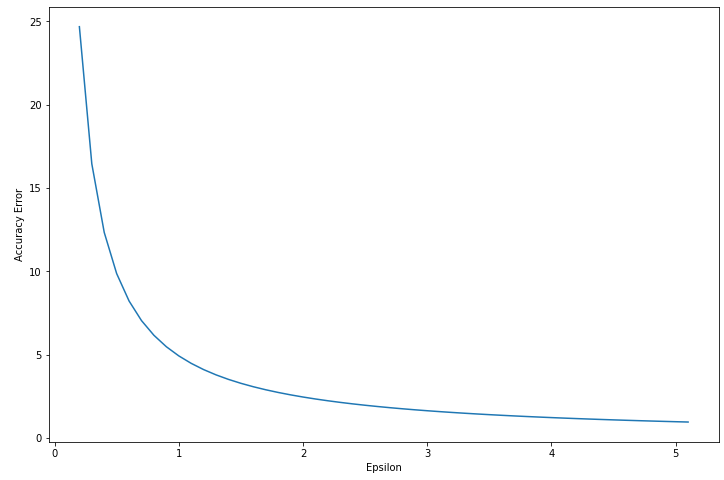
\includegraphics[width=0.6\textwidth]{images/epsilon_intro_graph.png}
  \caption{Accuracy Error as a function of epsilon}
\end{figure}

\section{Different forms of Differential Privacy}

As mentioned during the definition, due to the room that is left for its interpretation, there can be many forms of Differential Privacy. There are two major fields recognized, the \textbf{Global D.P.} and the \textbf{Local D.P.}.

Their major difference is the curator of the data. In the Global model, the curator must be trusted, as he collects the non-private data and has to pass them through a D.P. algorithm.

On the other hand, in the Local model, the curator may as well be untrusted, since the users perturb their data on their own, using a specific protocol. The key differences of the two forms are shown in the \textbf{Figure 2.2} below.

An other difference between the two models, is the amount of noise added. With the absence of a trusted curator, the users themselves must add a significant amount of noise into their data, in order to preserve their privacy. This of course results into a need of many users (several thousands), in order for the L.D.P. protocols to function correctly and accurately.


\begin{figure}[!htb]\centering
      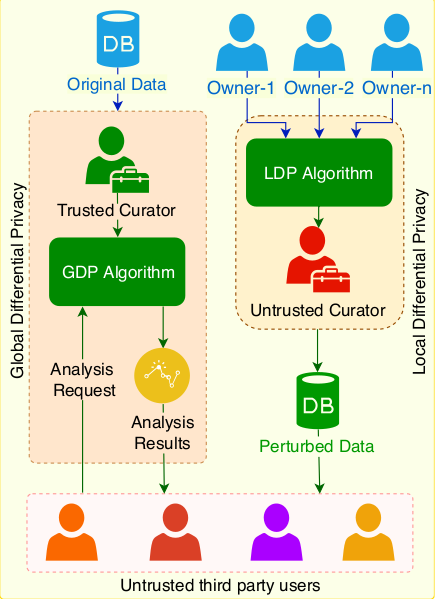
\includegraphics[width=0.3\textwidth]{images/local_vs_global.png}
  \caption{Differences between LDP and GDP}
\end{figure}

In this thesis, we are going to examine both models, by quoting their definitions, observing already-existing algorithms, and creating our own L.D.P. protocol.

\section{Existing Problems of D.P.}

As every new step in Computer Science, Differential Privacy has some issues that are yet to be solved, and some others not covered by its definition. 

One major problem is the behaviour of the protocols \textbf{when the number of users is limited}. The definition of D.P. is based on the alteration of the data in order not to reveal sensitive information. Thus, if a small amount of users are involved in those protocols, the accuracy of the results might be way off the standards that we set, in order to satisfy the epsilon requirements of the user.

Another (unsolvable) issue, that mainly lies on the basis of surveys, is  \textbf{the possibility that conclusions drawn from a survey may reflect statistical information about an individual}.

For example, if a survey about the correlation of smoking and dental problems is conducted, someone that has specific dental problems might be deemed as a smoker, despite keeping his privacy about the fact that he is smoking, during the survey. That is something that D.P. does not promise: unconditional freedom from distinguishing. This is not however a violation of the definition of D.P., as the survey teaches us that specific private attributes correlate with public observable attributes, since this correlation would be observed independent of the presence or absence of the individual in the survey.

There are several more issues as the ones covered above, however we are not going to focus on those, rather on the advantages of D.P.

\chapter{EXAMINATION OF PREVIOUSLY-EXISTING GLOBAL DP LIBRARIES}

The first goal of this Thesis is to examine previously existing programming libraries and APIs that provide the application of Differential Privacy to a dataset. This has been achieved by many companies, such as Google and IBM, but also from research programs like ARX that study the benefits of data privacy. We separate those implementations regarding their output. The possible outputs of a mechanism that adds D.P. to a dataset can be:
\begin{itemize}
    \item An answer to a query, in a private manner.
    \item An anonymized dataset, that meets the criteria of D.P.
\end{itemize}

In the first category, we can distinguish libraries such as Google's and IBM's, that have functions which if applied on a dataset, and given a specific query, can return a single answer.

In the second one, we can find libraries such as the ARX tool, that given a dataset and a group of privacy settings (such as the amount of noise to be inserted), produces an anonymized version of a dataset, that has obviously reduced information in comparison to the original one, but is usable by the final user.

In this chapter, we are going to test those libraries by providing different kinds of datasets, in order to determine the advantages and the disadvantages of each category.

We are going to conduct all of our testings using noise generated by the \textbf{Laplace Mechanism}, thus we must first define its theoretical behavior.



\section{The Laplace Mechanism}

The Laplace Mechanism is used widely in applications of Differential Privacy regarding \textbf{numerical queries}, which are actually functions that match a query to a number, or a vector of numbers, thus answering to it. The mechanism uses noise produced by the Laplace probabilistic distribution, which is equivalent to the query's sensitivity.

\subsection{Query Sensitivity}
The $l_1$ sensitivity of a query $f$, is defined as following:

\begin{align*}
    \Delta f = \max_{\{||x-y||_1 = 1\}} ||f(x) - f(y)||_1
\end{align*} where $x,y \in N^{|X|}$.

This quantity shows the effect by which a single participant's data can change in the worst case during the query $f$, and thus, the uncertainty that we must insert to to the response in order to protect them.

\subsection{The Laplace Distribution}
The Laplace Distribution with a scale $b$, is the distribution with probability density function: 
\begin{align*}
Lap(x|b) = \frac{1}{2b}exp(-\frac{|x|}{b})
\end{align*}

who's variance is $\sigma^2 = 2b^2$, and is actually a symmetric version of the exponential distribution.

\subsection{Use of Laplace in D.P.}

In order to be of use in our definition, the scale of the noise will be calibrated to the sensitivity of the query $f$, divided by epsilon. Thus, the noise used will be drawn from

\begin{align*}
Lap(\frac{\Delta f}{\epsilon})
\end{align*}

Of course, many other probabilistic distributions can be used to ensure differential privacy, but during our testings we prefer to use Laplace.

\section{Query Answering Libraries}

We are going to begin by testing libraries that belong in the first category, and specifically the \textbf{IBM's diffprivlib}, which is written in python, and is publicly available \href{https://github.com/IBM/differential-privacy-library}{here}. The library includes a host of mechanisms, the building blocks of differential privacy, alongside a number of applications to machine learning and other data analytics tasks. We are going to focus our testings in the simple queries, such as the \textbf{mean value}, the \textbf{extreme values} and the \textbf{histograms} of a numerical dataset. The library consists of three modules:

\begin{itemize}
    \item \textbf{Mechanisms}, as known from the theoretical foundations of D.P.
    \item \textbf{Models}, especially machine learning models, that will not concern us during this thesis
    \item \textbf{Tools} that will allow us to apply D.P. in datasets.
\end{itemize}

We are going to use the tools available, in order to apply differential privacy in a dataset of our own, guided of course by the mechanisms provided by diffprivlib. First, we are going to take a look at the dataset that we are going to use going forward.


\subsection{Setup of the mechanism}

The first step in order to test the library, is to setup the mechanism by defining its properties and parameters. 

\subsubsection{Bounds' Selection}

One of the most important aspects for us if we want to apply DP algorithms, is to define the bounds, i.e. the range that a variable can be in. It would be very convenient in our case to just take the tuple of the smallest and the largest value in the column that we are interested in. However, in the real world, the person who asks the queries is not supposed to know this info about the dataset. Thus, since a solution is not provided by the library, we must define our own bounds by guessing the lowest and the highest values in the fields that we want to examine. 

Thus, the user must have somewhat of a previous knowledge regarding the dataset, in order to decide the minimum and maximum value. Those values do not need to be precise, although the more close they are to real ones, the best the protocol will function. At the same time, we must be sure that during our selection we do not leave some of the dataset's values outside of the bounds, as they will be ignored in the final results. 


\subsubsection{Privacy Budget}

In this form of D.P., someone trying to breach the users' privacy, could theoretically ask an infinite number of questions, and thus each time gain more and more information about their private data. This is not covered by the definition of D.P., however it is not acceptable. In the same manner, an untrusted user of the library could ask the same question many times, aiming to determine how much noise is added each time, in order to find out the actual answer to the query, as the way that the noise is drawn is already known.

In order to eliminate this problem, a special parameter call the \textbf{privacy budget} is implemented. The library offers the ability to initialize this budget before asking any queries. During the queries, this budget is each time decreased, according to how much data the answer to the question reveals. For example, the answer to the "mean value of the charges for a surgery", costs less than the answer to the "histogram values of heart transplant surgeries in the West coast".

This parameter is implemented by the library as the budget accountant. This variable tracks the privacy spent, so that our system is not left exposed after lots of "expensive queries". The system will allow someone to ask one question that uses the whole privacy budget, or a series of questions whose total impact is less or equal to the initial budget.

\subsection{Testings' goal}

When applying D.P. mechanisms to our data, we provide the privacy settings of our choice (epsilon variable), and obtain an answer to each of our questions. Thus, in our testings, our goal is to \textbf{determine the accuracy of the answers}, given a specific ε, or some other settings, and comparing them to the true answer, using some metrics. Those metrics are different for each query type. In this section we are going to focus on two types of queries: statistical, and histograms.

\subsection{General techniques}
In each one of our following testings, we are going to run the query \textbf{many times}. As we already know, D.P. relies on probabilistic algorithms that can some times produce extreme results. This may be rare, but we want our testings and conclusions to be accurate. So, we are going to run each query 100 times, and return as a result the mean value of those runs.

\subsection{Statistical Queries}

The first type of queries that we are going to test are those that answer questions like "What is the mean cost of a surgery?", or "What is the largest fee paid by medicare for a transplant?", known as statistical queries. 

\subsubsection{Metrics used}

In the case of statistical queries, their answer is usually a real number, so in order to check their alteration with the true answer, we are going to take into account the \textbf{absolute difference between the truth and the query answer}. 

\subsubsection{Bounds Definition}

We are considering fees for surgeries in our example, thus a logical lower bound would be 0\$ (surgeries could be done pro bono too!), and an upper bound would be 1 million dollars. Either way, we are trying to be extreme with our picks, in order to not find ourselves in the unfortunate situation that a value taken into consideration by the DP query would be out of bounds.

\subsubsection{The identity of the testing Dataset}

The dataset chosen to test the library, is the publicly available "Surgery Charges Across the U.S.", that contains many different kinds of surgeries in a plethora of different hospitals. Our goal is to protect each hospital's data when it comes down to a specific surgery, while helping a patient choose one, depending on the charges that can be found all over the United States. The data provided in this dataset, is going to help a potential patient balance his need of top care, and the need to spend less money. The columns contained in the dataset are:

\begin{itemize}
    \item Surgery code and definition
    \item Provider hospital name
    \item Provider city
    \item Average total payments
    \item Average medicare payments
\end{itemize}

We are going to focus on the last two columns, in order to approximate the charges of a surgery. The above table gives us an image of the containers of the dataset.

The dataset contains a total of 200,000 entries, a more than satisfying number for running D.P. algorithms.

\begin{table}[!htb]

    \caption{"Surgery Charges Across the U.S." dataset columns}
    \label{numbers}

    \begin{tabular}{| c | c | c | c | c| c |}
      \hline 
      ID & Surgery Type & Hospital Name & Hospital City & Total & Medicare \\
      \hline
      1 & TRANSPLANT & MAYO CLINIC & PHOENIX & \$240422.80 & \$133509.55\\
      \hline
      2 & ECMO &  GROSSMONT HOSP & LA MESA & \$193617.86 & \$192003.43 \\
      \hline
      3 & CRANIOTOMY & STANFORD HOSP &  STANFORD & \$32597.87 & \$29347.12  \\
      \hline
    \end{tabular}

\end{table}

\subsubsection{General Dataset Utilities Queries}

Our first experiment is just to ask for some of the utilities of the dataset, and specifically its cost column: the \textbf{mean value}, the \textbf{variance}, the \textbf{sum} and the \textbf{standard deviation} values of the surgeries' cost. 

All of those queries can be executed using the following command (specifically for the mean value query):
\bigskip

\begin{lstlisting}[language=Python]
mean_with_dp = dp.tools.mean(df["Average_Total_Payments"].tolist())
\end{lstlisting}
\bigskip

where the dataframe column is the one containing the cost of each surgery, and its values should be in a list in order for the library to function.

By running the above mentioned queries, we got the following results:


\begin{table}[!htb]
    \centering
    \caption{General Queries results for Surgeries Dataset}
    \label{numbers}

    \begin{tabular}{| c | c | c |}
      \hline 
      Query & True answer & Private Answer \\
      \hline
      Mean value & 13168.5 & 13167.3 \\
      \hline
      Sum & 262754253.1 &  262935459.3 \\
      \hline
      Variance & 262754253.1 & 261940796.5\\
      \hline
      Standard Deviation & 18855.1 & 25825.0\\
      \hline
    \end{tabular}

\end{table}


The answers are almost perfect, for example on the mean value, considering that the cost is thousands of dollars, and the error is just 1 dollar. The simplicity of the query just lies to the following instruction:

However, this is just a simple example, executed only once, hence it can not provide us with safe conclusions for the library. In order to do so, we are going to run more complicated examples moving forward.

\subsubsection{Lowering the Dataset size}

As we mentioned above, the entries that the dataset contains are a very large number, and we know as a fact that D.P. functions well when this is the case. How is the library going to respond though if the dataset size is smaller? We are going to run for 4 different values of epsilon, and get the results for an increasing number of entries, starting from 10, and moving to 2000. Thus, the X axis of each plot represents the increasing dataset size, the Y axis the accuracy error, and each plot has a title of the epsilon setting used for the measurements. We can see the results in the \textbf{Figure 3.1} below.

\begin{figure}[!htb]\centering
    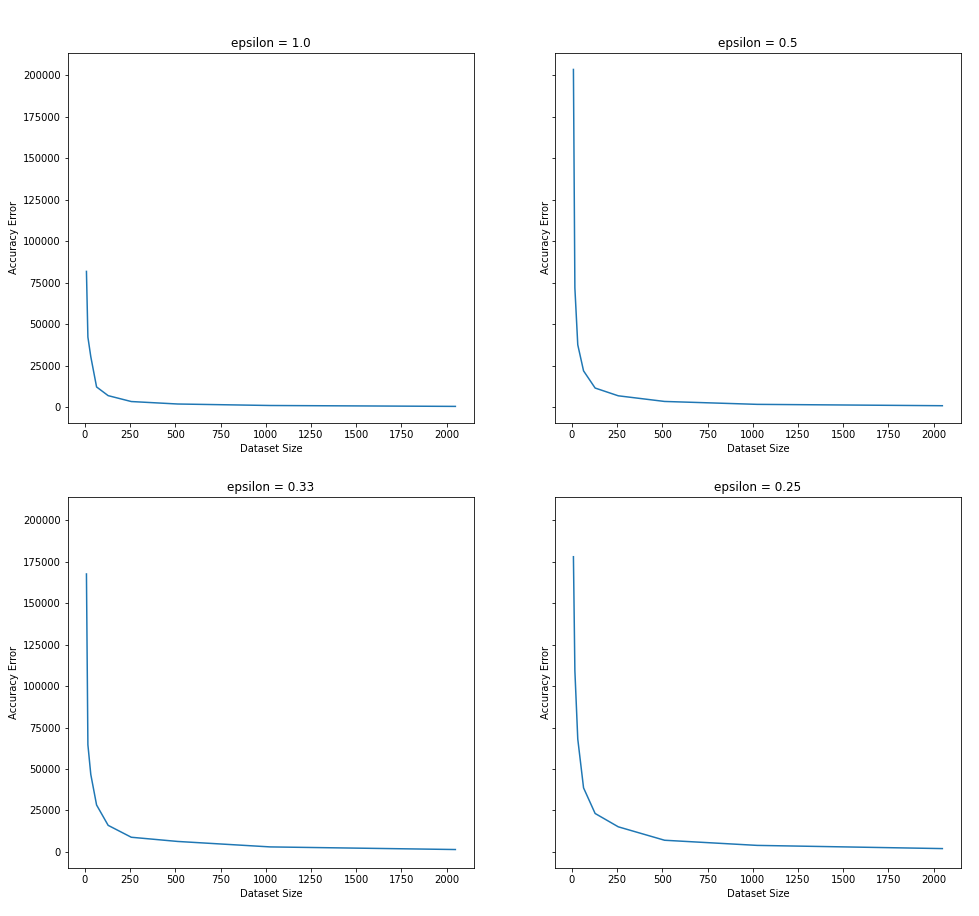
\includegraphics[width=1\textwidth]{images/increasing_ds_size.png}
    \caption{Accuracy Error for Increasing Dataset Sizes}
\end{figure}


By observing the plots, we can make a couple of conclusions:

\begin{itemize}
    \item \textbf{The smaller the epsilon gets, the bigger the accuracy error in the case of small datasets.} This, according to the definition makes sense, because small epsilon indicates higher privacy, thus for small datasets it can mean lower accuracy, due to the high amount of noise added.
    \item \textbf{The accuracy error stabilizes near 0 as the size of the dataset gets over 1000 entries.} Of course, depending to the epsilon value, this point could be earlier in the dataset sizes, as we observe for ε $= 1$. This again lays in the above mentioned property of the definition.
\end{itemize}

\subsubsection{Epsilon measurements}

The most important aspect when applying Differential Privacy to a dataset, is the selection of epsilon. This number is held accountable of the trade-off that DP offers: how much accuracy are we going to sacrifice in order to have less privacy loss, and vice versa. Given the library and our surgeries' costs dataset, we are going to measure the accuracy changes with the selection of different epsilon values.

The size of the dataset is too big, and thus the computation of the sensitivity will take too long. We assume that the data are somewhat equally distributed, thus we chose only 1\% of the dataset (which is a significant number of members), to take part in our sensitivity calculations.

In order to observe if the library functions well, we are going to compare the results produced with the \textbf{theoretical bounds of the Laplace mechanism}. 

In theory, the accuracy of an ε-differential private query, can be at most equal to the sensitivity of the query divided by epsilon, thus $$\frac{\Delta f}{\epsilon}$$ where $\Delta f$ denotes the sensitivity, and ε is our current privacy setting. 

Sensitivity is defined as the maximum difference that can be found if we alter a single entry in the dataset. We can define 2 types of sensitivity:

\begin{itemize}
    \item \textbf{Local Sensitivity} which in theory is $ \Delta f = \max_{||x-y||_1 = 1} ||f(x)-f(y)||_1$
    \item \textbf{Global Sensitivity} which we are going to use in our testings, and is defined as:
    \begin{align*}
        \Delta f = \frac{upper - lower}{length(DB)}
    \end{align*} where upper and lower are the highest and lowest values of the column we are interested in our dataset, and length is the size of the database.
\end{itemize}

In order to compute the local sensitivity, we must check the maximum difference in the query result that occurs if we remove a single person from the database. We are going to define a function to do so, so we can check the theoretical bounds during our tests.

The results of those testings are shown in the \textbf{Figure 3.2}.

\begin{figure}[!htb]\centering
    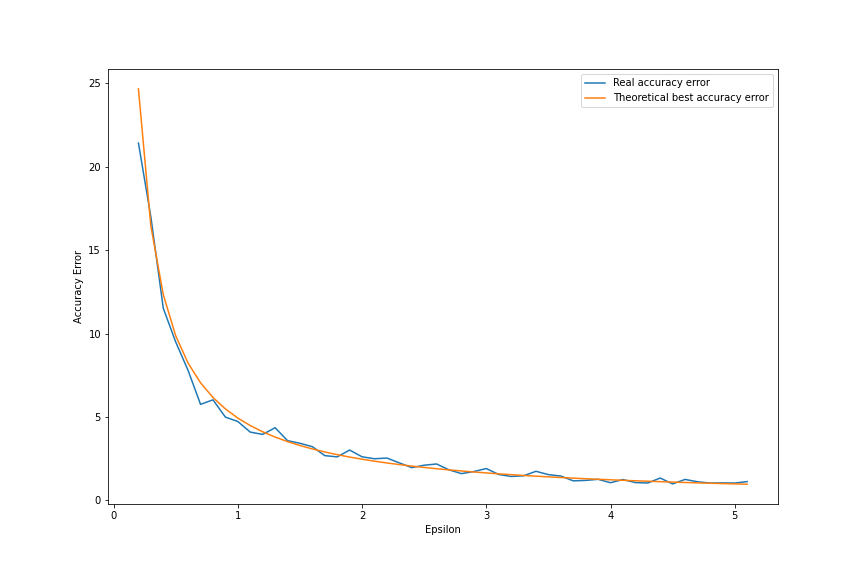
\includegraphics[width=1\textwidth]{images/epsilon_measurements.png}
    \caption{Real and Optimal Accuracy Error for Increasing epsilon values}
\end{figure}

It is clear that as we increase the epsilon value, the privacy loss gets bigger. On the other hand, if epsilon is too small, as we can see in the above plot, extreme errors in accuracy in our queries will emerge. 

The optimal value of epsilon varies, there is no general rule for the perfect epsilon. It depends on many different aspects, such as:

\begin{itemize}
    \item The noise generated by the probabilistic mechanism used
    \item The implementation of the algorithm
    \item The size of the dataset
    \item The query itself.
\end{itemize}

Moreover, the selection of epsilon depends on the dataset. For example, we might have a dataset that is extremely important to have minimal privacy loss. In that case, we will opt to use a rather small epsilon, thus we do not disclose the sensitive data included. An other dataset could be less sensitive, but the analyst might have a need for extreme accuracy every time, so the epsilon selected should be rather big.

Regarding the comparison with the Laplace bounds, we can see that the library's query performs significantly well throughout the different epsilon values selected. This is due to the fact that IBM uses the same formula to compute the sensitivity, as well as a similar mechanism (Laplace truncated noise), in order to answer to our queries.

\subsection{Histogram Queries}

Histogram graphs are a very handy way to visualize numerical data, compare different values of a specific field, and thus extract conclusions about the dataset. We are going to study the `diffprivlib`'s method of creating an histogram, and its accuracy when changing the epsilon factor.

The IBM DP library offers a differential private way to create histograms. The difference with the simple queries that we tested, is that now, \textbf{geometric truncated} noise is added in order to satisfy DP.

\subsubsection{Metrics Used}
The result of a histogram query on a dataset is a vector containing how many entries belong on a specific range. Thus, the comparison between 2 histograms can be held out by comparing those vectors. 

There are plenty of metrics used to compare vectors, but we are going to focus on the \textbf{Euclidean Metric} and the \textbf{Kantorovich metric} (also known as Wasserstein or EMD metric). 

The Euclidean metric is one of the most simple metrics, as it takes into account the distance between each pair of the two vectors. Thus, the distance of the vectors is defined by:

\begin{align*}
    d = \sqrt{\sum_{i=1}^n (x_i - y_i) ^ 2}
\end{align*}

where $n$ are the total elements of the vectors (must be of equal size), and $x$ and $y$ are the 2 vectors that we are comparing.

The Kantorovich metric is a more complex one, as it examines the cost to move a specific quantity of the one vector to the other, in order for the two to be similar, and thus figuring out their distance. For example, the Kant. distance is larger if we have the vectors $[0 0 0 1]$ and $[1 0 0 0]$ than having the vectors $[0 0 0 1]$ and $[0 0 1 0]$, as in the first case the first element of the histogram is moved 3 places in order to be similar to the second one. In order to determine the cost, a base metric is used, which in our case will be the euclidean.

The way that the metric works in a naive approach, is explained in \textbf{Figure 3.3.}

\begin{figure}[!htb]\centering
    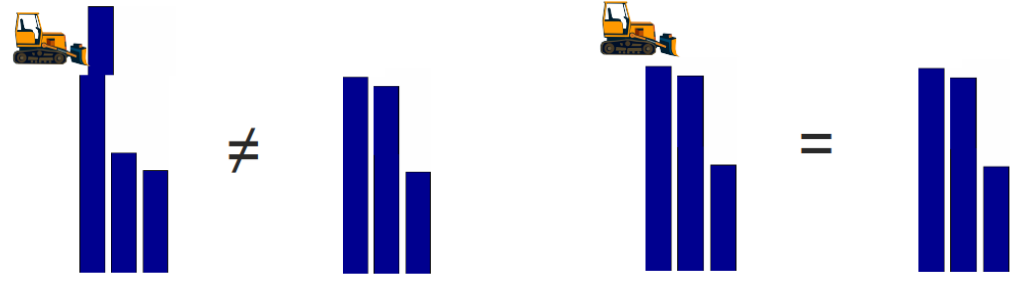
\includegraphics[width=0.7\textwidth]{images/emd.png}
    \caption{Kantorovich Metric Application on 2 histograms}
\end{figure}

This metric is much more suitable for D.P. as we are not just interested in the alteration of the results, but on the amount of alteration. If, for example, we are examining a histogram that contains the age of a hospital's patients, it is not the same for the private histogram to deem a 10 year old patient as 90 year old, than deeming him as 11. 

In order for the Kantorovich metric to be computed, we must solve a Dynamic Programming Problem, and make complex calculations, which are beyond the subject of this thesis. There are many implementations of the metric, and since IBM's library is written in Python, we are going to use the QIF library %TODO:Insert mention.
which is also available as a Python library. 


\subsubsection{Bounds Definition}

In the following testings we are examining salaries, thus we must set the lower and the higher bounds such as to support the most extreme salaries that could possibly be present in the dataset. Therefore, the lower bound is set to 0 dollars, and the higher to 500,000 dollars.

\subsubsection{The identity of the testing Dataset}

During our histogram testings, we are going to use a different dataset, which contains  sensitive data regarding employee's salaries in the state of Baltimore, while stating other facts about the members of the dataset. 

The columns contained are: 
\begin{itemize}
    \item Name
    \item Job Title
    \item Annual earnings
    \item Gross earnings
\end{itemize}

We are going to focus on the last 2 columns, containing the employees' salaries. The dataset has 13000 entries, which are more than enough in order for our histograms to be realistic and accurate. The above table gives us an image of the containers of the dataset.

\begin{table}[!htb]
    \centering

    \caption{"Baltimore State Employees Salaries" dataset columns}
    \label{numbers}

    \begin{tabular}{| c | c | c | c |}
      \hline 
      Name & Job Title & Annual Earnings & Gross \\
      \hline
      Aaron,Kareem D & Utilities Inst Repair I	 & 32470.0 & 25743.94 \\
      \hline
      Abadir,Adam O	 & Police Officer &  60200.0 & 57806.13  \\
      \hline
      Abbeduto,Mack & Council Technician & 53640.0 &  59361.55 \\
      \hline
    \end{tabular}
\end{table}

\subsubsection{Simple queries}

At first, we are going to run simple instances of histogram queries, so we can take a look at the amount of error that we expect moving forward, and also familiarize with the execution of the commands. To create a private histogram using the library, we must provide the bins. Those should be identical to our bounds, that we have earlier defined. While creating the non-private histograms we are going to use the same bounds, in order for our comparisons to make sense. The creation of the bins and the private histogram are achieved using the following Python instructions:

\bigskip
\begin{lstlisting}[basicstyle= \footnotesize,
language=Python]
bins = np.linspace(0, 300000, 20)[1:]
result = dp.tools.histogram(input_list, bins = bins, 
         epsilon = epsilon, range=bounds_range)[0]
\end{lstlisting}
\bigskip

where epsilon is the float number selected as the epsilon parameters, and bounds range is the tuple of our dataset bounds.

The result of the execution of both the private and the non-private histogram queries for the annual earnings column are shown below, in the \textbf{Figure 3.4}.

\begin{figure}[!htb]\centering
    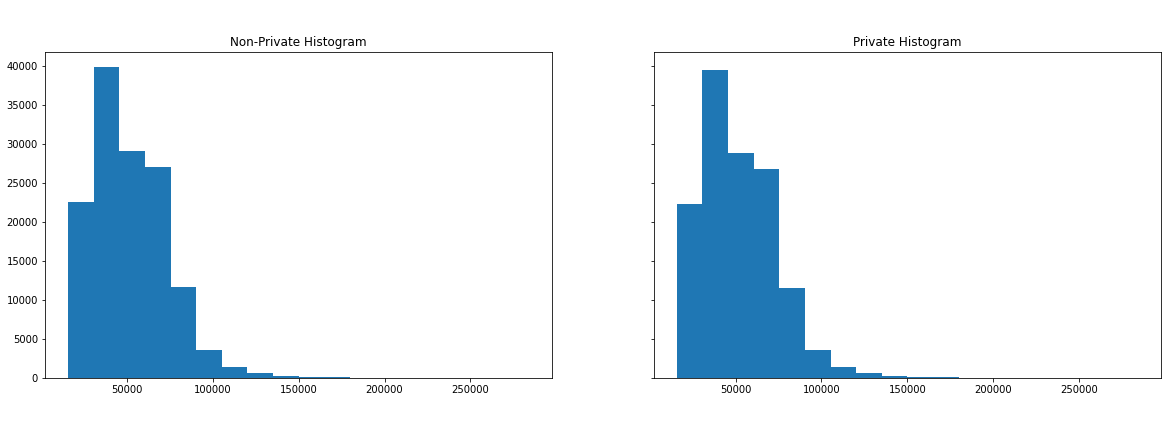
\includegraphics[width=1\textwidth]{images/simple_hists.png}
    \caption{Private and Non-private histograms for the Salaries Dataset}
\end{figure}

The results are more than satisfying in the naked eye. This is probably due to the large dataset size: we are not able to locate small changes. In order to do so, we are going to check our error using the accuracy error function that we have defined.

While applying our metrics, the Euclidean error is $14.81$, and the Kantorovich error is $91.63$. The euclidean distance error determines how many entries were wrongly classified in a bin (in average), when the differentially private query was run. So, less than 20 people out of 13.000 were wrongly classified, whereas their privacy was secured. This is quite a good trade-off!

\subsubsection{Epsilon Measurements}

Once again, we are going to run the histogram queries for different values of epsilon, in order to check their behavior as the parameter increases. The results of the execution for the Euclidean metric are shown in the \textbf{Figure 3.4}, and for the Kantorovich metric in the \textbf{Figure 3.5}. 


\begin{figure}[!htb]\centering
    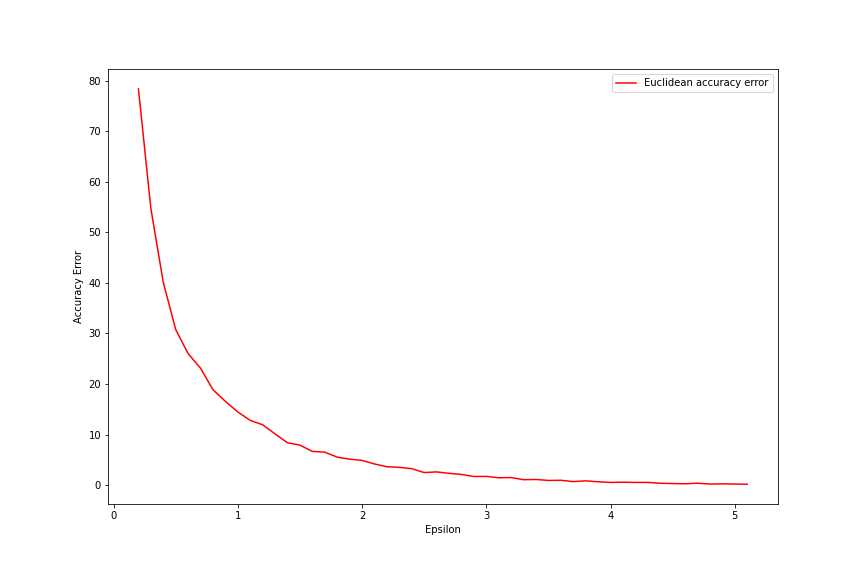
\includegraphics[width=1\textwidth]{images/hist_metrics_euclidean.png}
    \caption{Euclidean Metric Error for increasing values of epsilon}
\end{figure}

\begin{figure}[!htb]\centering
    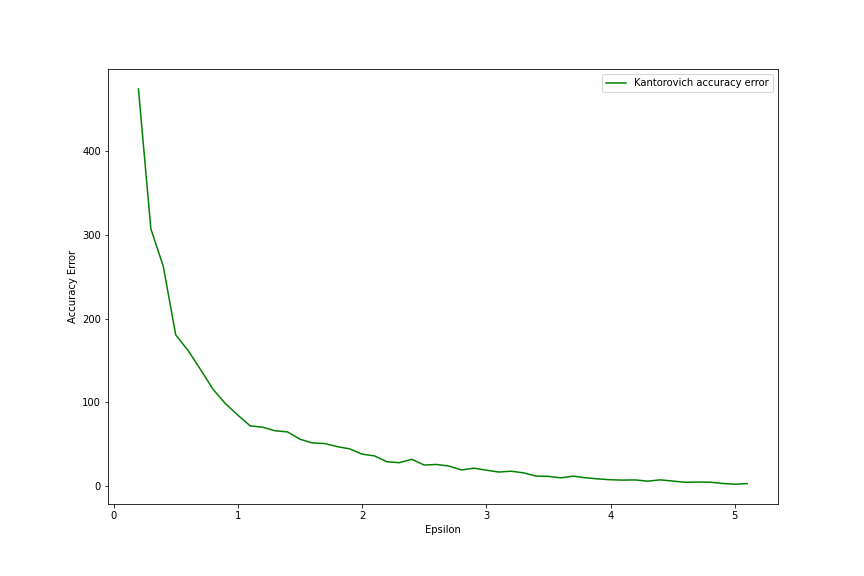
\includegraphics[width=1\textwidth]{images/hist_metrics_kantorovich.png}
    \caption{Kantorovich Metric Error for increasing values of epsilon}
\end{figure}

We observe that the error curves follow the same ratio as the previous ones, indicating what we already know, that the error decreases as the epsilon values increase. This is another case where the library produces accurate and definition-aware results. 

\subsubsection{Histogram queries in theory}
Based on [1] the histogram queries are very high sensitivity queries, thus a slight change to the bounds could be critical for their result. 

The authors suggest that we use noise generated by the LaPlace mechanism, but with a slight change. In detail they suggest the following:

\textit{"In the special (but common) case in which the queries are structurally disjoint we can do much better — we do not necessarily have to let the noise scale with the number of queries. An example is the histogram query. In this type of query the universe $N^X$ is partitioned into cells, and the query asks how many database elements lie in each of the cells. Because the cells are disjoint, the addition or removal of a single database element can affect the count in exactly one cell, and the difference to that cell is bounded by 1, so histogram queries have sensitivity 1 and can be answered by adding independent draws from $Lap(\frac{1}{\epsilon})$ to the true count in each cell."}
\clearpage

\subsection{Conclusions}

After a rather satisfying amount of testing in a large, real world dataset, we can safely say, that the IBM DP library has quite impressive results when it comes down to the trade-off between privacy and accuracy during both simple counting queries and histogram ones. However, we are cautious about 2 problems that were observed while using the library:

\begin{itemize}
 \item \textbf{Bounds checking}. The user must define himself the bounds, a fact that causes for speculations on the variance of the values in the dataset. It would be convenient to take the lowest and highest value in the field that we are examining, in fact that is how IBM demonstrates those examples, but that violates the rule that prevents the user from having any info of the dataset before the DP processing.
 
 \item \textbf{Non-DP preprocessing}. If we ask complicated queries (ex Surgeries performed in Stanford), the library does not offer a way to preprocess the data, thus we trust python in doing so, which results in a non-DP way of shrinking the dataset. The result obtained is of course differential private, but what happens if the dataset has only 1 record in it? That, while being a very extreme case, violates the definition of differential privacy.
\end{itemize}

The bounds' problem can be solved by running a minimum and maximum value differentially private query, which might in some cases leave certain datasets out, but is a rather satisfying solution. 

The Non-DP preprossessing is a more tricky one, that needs special techniques in order to cover the edge case mentioned. However, we are going to check such techniques in the following section, which is based on returning the whole dataset after the application of D.P.



\section{Anonymized Dataset Producing Libraries}

As mentioned earlier, an other possible output of a mechanism that adds D.P. to a dataset can be the dataset itself, after being anonymized using certain algorithms that meet the criteria of D.P.

This technique does not yet have many different implementations, mostly due to the success of the previous model shown, as well as the difficulty, the computer power needed and the poor quality of the result being produced.

Producing an anonymized dataset is the way to go if someone is using earlier forms of data privacy, such as \textbf{k-anonymity}, \textbf{l-diversity} etc, which we are going to analyze moving forward. However, in order to cover the needs of D.P., several adjustments have to be made. The main idea behind all those libraries, lay behind a theorem, presented in [TODO: insert ref paper], that mixes the use of those previously mentioned techniques with D.P.

In this Thesis, we are going to examine the \textbf{ARX tool}, a tool for data anonymization, that supports the method that we are trying to implement. We are going to analyze this tool, and perform similar testings as in IBM. ARX is a tool for data anonymization, that in general, takes a dataset as an input, applies  privacy models, and produces an anonymized version of this dataset, thus offering protection to its members. The Menu of the ARX tool can be seen in the following Figure 3.7.

\begin{figure}[!htb]\centering
    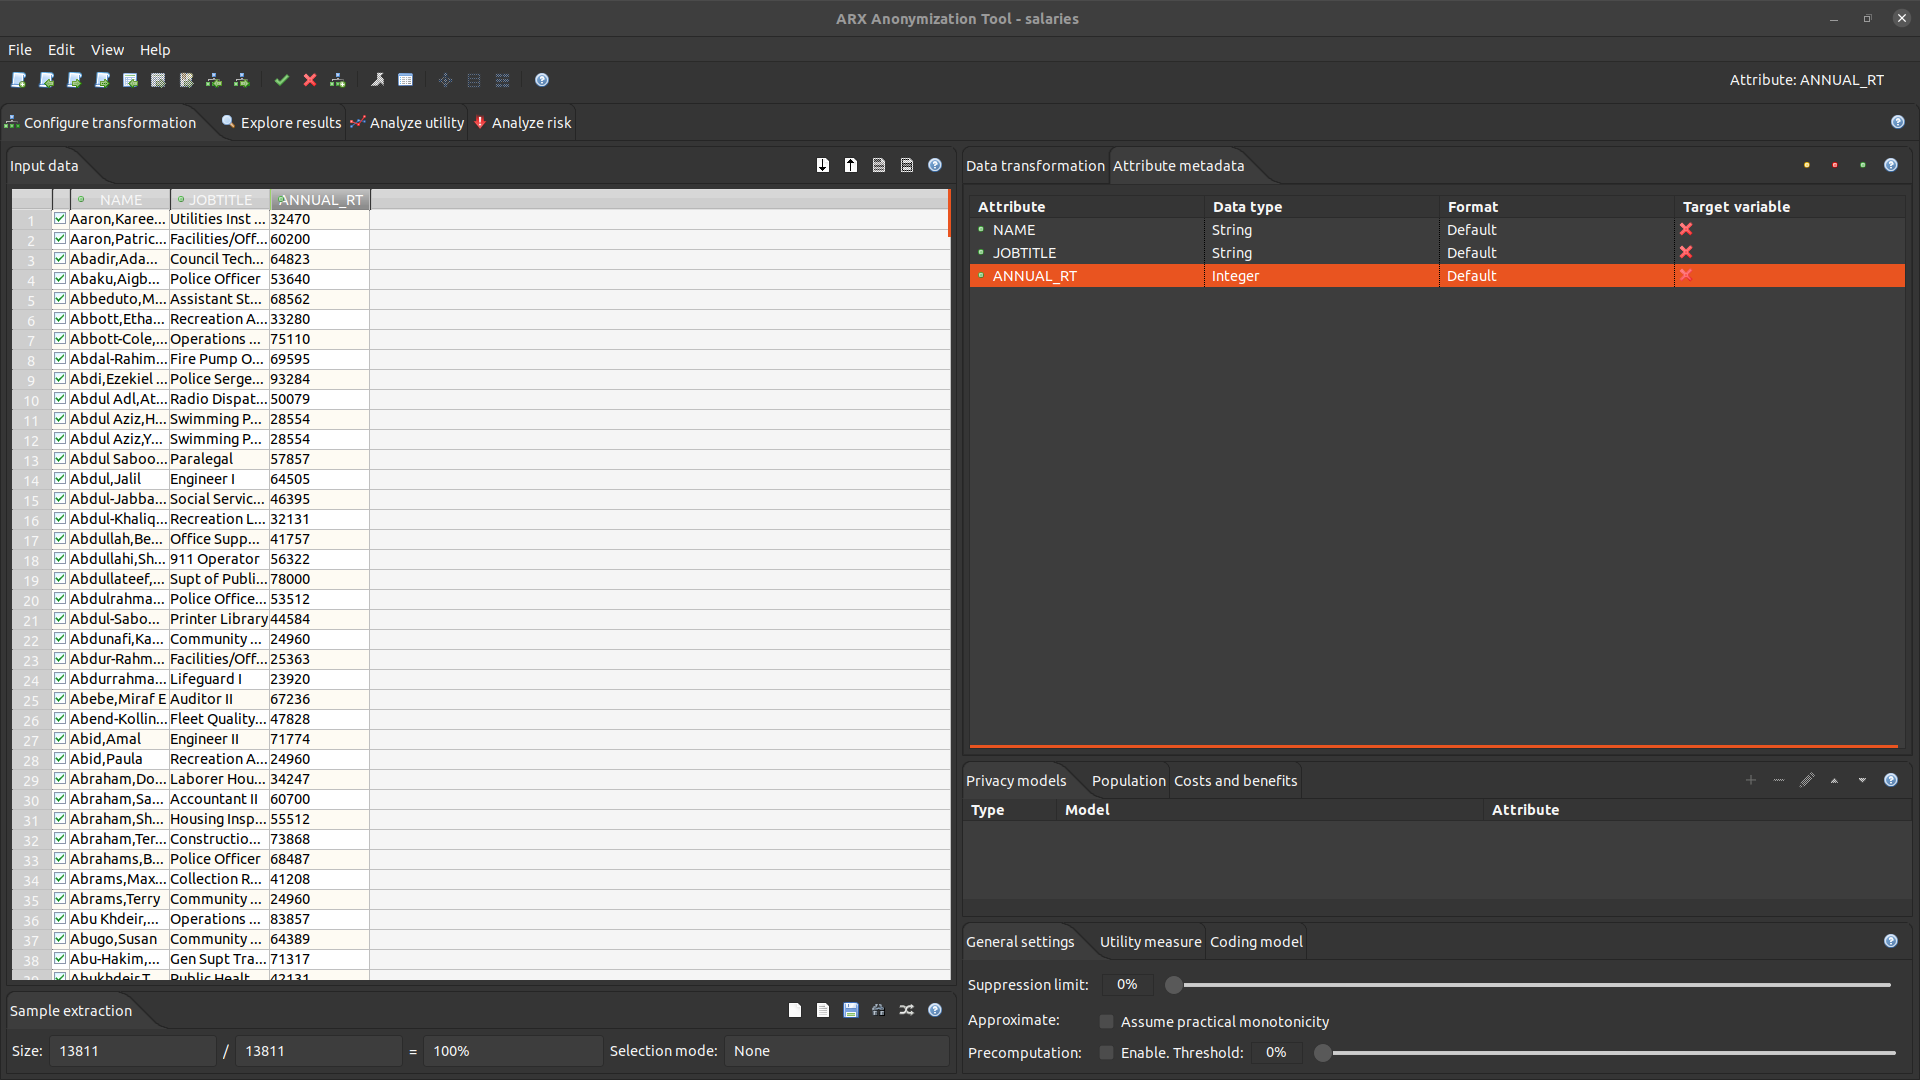
\includegraphics[width=0.9\textwidth]{images/arx_tool.png}
    \caption{The ARX GUI tool}
\end{figure}

At its core, ARX uses a highly efficient globally-optimal search algorithm for transforming data with full-domain generalization and record suppression. The transformation of attribute values is implemented through domain generalization hierarchies, which represent valid transformations that can be applied to individual-level values.

\subsection{Classic Privacy Models}

The ARX tool offers standard privacy models that are tested in theory and are widely use to ensure anonymity given a plain dataset. Those consist of the implementation of the following protocols:

\begin{itemize}
    \item \textbf{K-anonymity}: A well-known privacy model that aims at protecting datasets from re-identification in the prosecutor model. A dataset is $k$-anonymous if\textbf{ each record cannot be distinguished from at least $k-1$ other records regarding the quasi-identifiers.} Each group of indistinguishable records forms a so-called equivalence class. 
    \item \textbf{l-diversity}: This privacy model can be used to protect data against attribute disclosure by ensuring that each sensitive attribute \textbf{has at least $l$ "well represented" values in each equivalence class}. Different variants, which implement different measures of diversity, have been proposed.
\end{itemize}

Moreover, the tool uses some simple concepts of processing a dataset:

\begin{itemize}
    \item \textbf{Random Sampling}: A probability sampling method is any method of sampling that utilizes some form of random selection. In order to have a random selection method, we must set up some process or procedure that assures that the different units in your population have equal probabilities of being chosen.
    \item \textbf{Attribute Generalization}: Generalizing a column of the dataset, based on its values. The applications of attribute generalization depend on the type of records(eg. integers, ranges etc).
    \item \textbf{Record Suppression}: Deletion of a specific row on the input dataset.
\end{itemize}

Those are some techniques that are not going to be analyzed and tested in this thesis, however, if combined with D.P. can produce interesting results. Specifically, according to [TODO:insert cite], the following theorem applies:

\textbf{Random sampling} with probability $\beta$ followed by \textbf{attribute generalization} and the \textbf{suppression} of
every record which appears less than k times \textbf{satisfies $(\epsilon, \delta)$ differential privacy} for every $\epsilon \geq -ln(1-\beta)$ with 
$$\delta = \max_{n:n \geq n_m} \sum_{j>\gamma_n}^{n}f(j;n,\beta)$$

where $n_m = \frac{k}{\gamma} - 1$, $\gamma = \frac{e^\epsilon-1+\beta}{e^\epsilon}$ and $f(j;n,\beta) = {n \choose  j} \beta^j(1-\beta)^{n-j}$.

In order to achieve attribute generalization, ARX uses the so called \textbf{hierarchies}. They are either imported from a csv file, or being hard-coded into the API, and they are used in order to generalize a sensitive field. An example is given in the Table 3.4. The subject to generalize is the age of a person. Let's see the values as they proceed through generalization.

\begin{table}[!htb]
    \centering

    \caption{"Baltimore State Employees Salaries" dataset columns}
    \label{numbers}

    \begin{tabular}{| c | c | c | c |}
      \hline 
      $1^{st}$ level & $2^{nd}$ level & $3^{rd}$ level & $4^{th}$ level\\
      \hline
      1 & 0-4 & 0-9 & *\\
      \hline
      3 & 0-4 & 0-9 & *\\
      \hline
      5 & 5-9 & 0-9 & * \\
      \hline
      10 & 10-14 & 10-19 & *\\
      \hline
      18 & 15-20 & 10-19 & *\\
      \hline
    
    \end{tabular}
\end{table}

\subsection{Conducting D.P. Testings}

ARX provides a cross-platform graphical tool, that supports many different ways of anonymizing data, as well as an API that delivers those data anonymization capabilities to Java programs. We are going to use the latter, in order to create our own scripts for testing the tool and its accuracy.

In order to test the accuracy of the models used by ARX, we are going to run simple queries, on the datasets produced by the anonymization process. We want to eliminate the probability of extremely high noise generation, thus we are going to run the anonymization tool multiple times, and the output dataset will be constructed by the mean values of the fields.

As show on the above matrix, ARX hierarchies tend to treat every type of value as a string, in order to replace it with a interval. This is not  desirable when applying the testings we mentioned. Thus, we had to come up with a better solution of defining hierarchies. The ARX GUI provides a wizard that gives a variety of choices so the user can easily create a hierarchy for plenty data types.

Another challenge is the number of layers that we are going to use, meaning how far our anonymization will proceed. In each layer, the number of same records increase exponentially, thus we do not want to apply many layers, in order for our results to be accurate, and the output dataset to be readable.

Given the help from Dr. Fabian Prasser, one of ARX's creators, we opted to treat the integer values as numbers, and in each level:
\begin{itemize}
    \item Group the rows by 2
    \item Apply a function according to the query we want to ask.
\end{itemize}
 
For example, if we want a counting query, the best option would be to apply an \textbf{arithmetic mean} function to the group, thus the sum, the mean, the variance etc will be the same. The way that ARX preserves D.P. with those settings, is by record suppression. If that was not the case, the results would be identical to the input dataset. However, now, the output dataset will differ because of its lack of some rows of the input.
 
Regarding the layers problem, we opted to use 4 layers of anonymization, the last of whom will be the * value, meaning that every record is inseparable. We do not want this to happen early in our anonymization, but we do not want it to never happen either, because then we would have a privacy leak, if the dataset was too small.

The creation of the hierarchies for the salary column, can be shown in the Figure 3.8, taken from the ARX GUI Hierarchy Creation Wizard.

\begin{figure}[!htb]\centering
    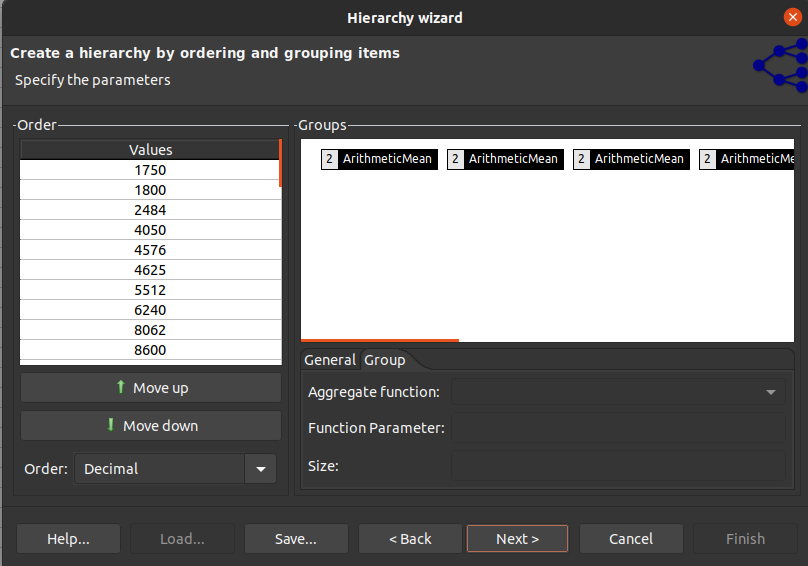
\includegraphics[width=0.8\textwidth]{images/hierarchies.png}
    \caption{Creating an Hierarchy using ARX GUI}
\end{figure}


\subsection{Metrics Used}
We are going to test the applicability of the already given ARX mechanisms on a numerical dataset. Our goal is to run basic queries, such as mean value on the dataset's records. We are going to do that first by applying no DP at all, and then by using the API that is presented by ARX, helped by a simple java script that was built for this purpose.


\subsection{The identity of the testing Dataset}
The dataset that we are going to be looking at, contains sensitive data regarding NBA players' \textbf{salaries} from the year 1990 until today. It also states other info about them, such as their \textbf{age}, their\textbf{ current team }and their \textbf{position}. This particular data is not considered sensitive, as those numbers are widely available, however, when it comes down to certain people's salaries, applying D.P. in order to preserve privacy is crucial.

\subsection{Process of running the queries}
As we have earlier noted, the application of D.P. in ARX is rather complicated, let along the use that we are interested in: We want the output dataset to have numerical values in the earnings' column, in order to apply queries. 

For each column of the dataset, we have defined our own hierarchies. For every column except the `Salaries` one, this hierarchy is semantic, like the ones presented in our intro for age.

For the salaries column, with it being our goal to analyze, we opt to use the construction mentioned in our solution in the intro. We created 7 layers, in order to give the algorithm the ability to anonymize the dataset without the values being converted to `*`.

A sample of the result of the creation of the Salaries hierarchy is presented in the above table, and the whole file is available in the GitHub distribution of the results of this Thesis.

\begin{table}[!htb]
    \centering

    \caption{Hierarchy Levels created}
    \label{numbers}

    \begin{tabular}{| c | c | c | c | c|}
      \hline 
      $1^{st}$ level & $2^{nd}$ level & $3^{rd}$ level & ... & $7^{th}$ level \\
      \hline
        79.568  &	291.029 & 500.776 &   	... &	*\\
              \hline
        502.491 &	291.029 &	500.776 &... &	*\\
              \hline
        522.738 &	710.524 &	500.776 &...	&   *\\
              \hline
        898.310 &	710.524 &	500.776 &... &	*\\
              \hline
        1.000.000 &	1.114.013 &   1.220.739 &...&	*\\
              \hline
        1.228.026 &	1.114.013 &   1.220.739 &... &	*\\
              \hline
    \end{tabular}
\end{table}

Next up, we are going to setup the use the ARX API, which requires us to specify some variables in order to run Differential Privacy. Those variables are defined in the above Java code, and are those that were use in the actual testings.

\bigskip
\bigskip
\bigskip
\bigskip
\begin{lstlisting}[
basicstyle= \footnotesize,
language=Java]
    EDDifferentialPrivacy criterion = new EDDifferentialPrivacy(2d, 1d / Rows);

    ARXConfiguration config = ARXConfiguration.create();
    config.addPrivacyModel(criterion);
    config.setSuppressionLimit(1d);
    config.setHeuristicSearchStepLimit(100);
    ARXResult result = anonymizer.anonymize(data, config);
\end{lstlisting}
\bigskip


The basic principles that were followed for the above definitions are based on the following instructions and guidance by the ARX tool documentations:
\begin{itemize}
    \item The delta value should not be 0, but is suggested to be set lower or equal than the reciprocal of the number of records.
    \item A suppression limit should be set, preferably to 1.
    \item In order to improve the quality of the data produced, a heuristic search step limit should be set, in order to tweak the ARX search algorithm that handles data suppression.
\end{itemize}

Additionally, following the same principles as with the IBM library, we are going to run the D.P. query multiple times before reporting its value. We are going to do so, because the amount of noise generated can be extreme, and because of the low bounds of the heuristic search that we have set. We chose to run each query 1000 times, and then report the mean value of those runs as the result produced by the mechanism.

Because of the structure of the result of the ARX mechanism (a dataset containing numerical values), we can only run queries like \textbf{sum} and \textbf{mean}. There is no point in running a min or max query: we already know that the result will not be accurate. Thus, we are going to try to run a\textbf{ mean value} numerical query in the anonymized dataset. The function we are using in order to run this typed of queries is the following:
\bigskip
\clearpage
\begin{lstlisting}[
basicstyle= \footnotesize,
language=Java]
protected static double run_query(ARXResult data, int targetColumn) {
	// iterator that we are going to use to access the data
	final Iterator<String[]> itHandle = data.getOutput().iterator();
	
	// result of the query
	double result = 0d;
	// length of the dataset
	int totalRecords = 0;
	
	// ignore the name of the column
	String[] name = itHandle.next();
	if (name.length <= targetColumn) {
		System.out.println("Target column out of bounds\n");
		return 0d;
	}

	// iterate through all the values in the dataset
	while(itHandle.hasNext()) {
		String[] next = itHandle.next();
		// check that our target position is legal
		String string = next[targetColumn];
		if (!string.equals("*")) {
			result += Integer.parseInt(string);		
			totalRecords++;				
		}
	}
    // return the __mean__ of the dataset
    return result / totalRecords;
}
	
\end{lstlisting}
\bigskip

Finally, before running the queries, we must mention that the dataset size should be significant, as our own contains thousands of columns. The dataset size is a critical parameter when applying D.P., while being even more essential during the use of the ARX tool.

\subsection{Statistical Queries}

As shown by the above Java function, our testings can support every type of statistical queries, such as \textbf{mean value}, \textbf{sum}, and \textbf{average}. However, we due to the computer power required and the similarity of the results that those queries produce, we will focus our testings solely to the mean value query.

Given the dataset previously analyzed, the true value of the mean value of the salaries column of the dataset is $\$2.868.981,32$. This will be the value that we are going to use in order to find out the accuracy of the D.P. results.

\subsubsection{Running with fixed parameters}

We are going to conduct our first test by anonymizing our dataset using the default parameters, as we set ε $ = 1$ and δ $ = \frac{1}{12377}$.  The results are shown in the following table.


\begin{table}[!htb]
    \centering

    \caption{Mean value query in ARX with default parameters}
    \label{numbers}

    \begin{tabular}{| c | c |}
      \hline 
        Non-DP result & DP Result \\
      \hline
        $\$2.868.981,32$ & $\$2.860.215,6$\\
      \hline
    \end{tabular}
\end{table}

We observe that the query results, are somewhat close: We are in the range of millions of dollars, and the ARX mechanism only fails to approach the result by 8 thousand. This is not of course close to what the IBM library computed, but it is still a reliable result, given all the downsides of this type of anonymization.


\subsubsection{Running with different epsilon values}

Next up, in order to determine if ARX follows the rules of D.P., we should try anonymizing the dataset for different values of epsilon, just like we did with the IBM library.

We observed during our initial runs that if the epsilon value rises above 2, the algorithm faces certain problems, that will be analyzed moving forward. With that being the case, the epsilon values chosen to conduct the measurements are in the range $[0.2, 1.6]$. The results from our testings are shown in the above Figure 3.8.

\begin{figure}[!htb]\centering
    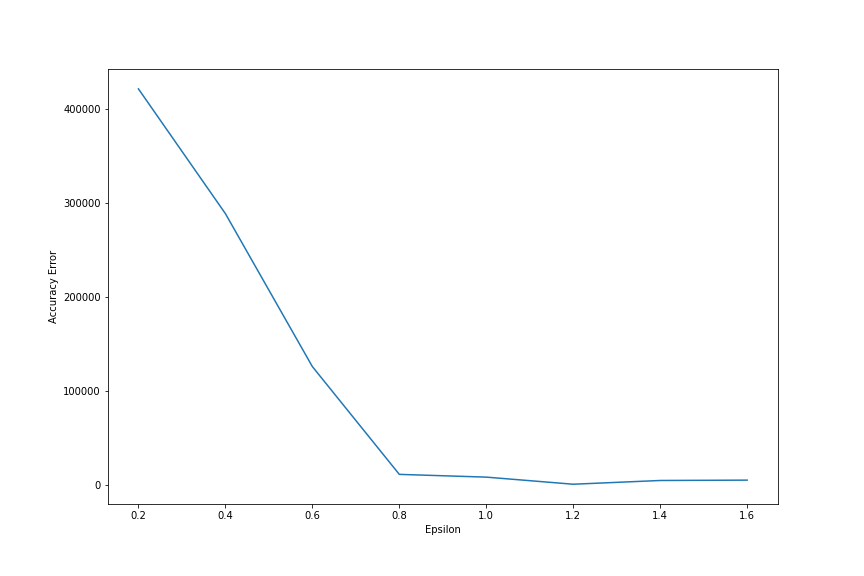
\includegraphics[width=1\textwidth]{images/arx_accuracy.png}
    \caption{Accuracy Error results for increasing values of epsilon}
\end{figure}

As we can see, the plot does not behave as expected, but it is in the right direction. We are used to seeing a more logarithmic-like plot, but here we observe that when the epsilon rises above `0.8`, the results are similar. We can not compare the results with the Laplace noise distribution, because of the way that the results are produced. 

We generate the answers given by asking the query in the output dataset. Without its records being suppressed, the result dataset would have been perfect, because of the transformation of the data. However, when suppressing many records (nearly 10\% each time), the result could be severely altered, and thus the error plot, as we saw, is quite unpredictable.


\subsection{Observations regarding the Algorithm}

During our testings in the dataset using the ARX mechanism, we observe the following regarding its behavior in the DP queries:

\begin{itemize}
    \item The epsilon variable if raised above 2,5, makes the algorithm \textbf{extremely slow}, to the point that it does not respond after minutes of execution. This makes sense, if we take into consideration that when epsilon increases, the accuracy gets better. Thus, the algorithm performs extreme searching techniques in order to find which records to suppress, resulting into slow execution.
    \item In order for the algorithm not to produce only *(the last level in our hierarchies) in our target column, we set each of the other columns as \textbf{non sensitive} in their definition.
    \item As the epsilon values rise, \textbf{the accuracy gets better}, as it is supposed to be, according to the DP principles.
    \item While the dataset has multiple columns, the algorithm usually fails to present all of them with anonymized values, and just reports * in each row. This could have been a result of the high \textbf{Heuristic Search Step Limit}, which was by default set to maximum. Despite us lowering its value, the phenomenon persists.
\end{itemize}

\subsection{Conclusion}

While researching the ARX mechanism we came to the conclusion that it is for sure a whole different approach in Differential Privacy compared to the other libraries that we studied. With that being the case, it has some advantages and some disadvantages. Its main advantages are the following:

\begin{itemize}
    \item The result of the mechanism is a \textbf{handy dataset} that the user can handle in multiple ways and gain more information than just the result of a query.
    \item The result \textbf{can be iterated}, thus giving the option to the user to run the query in a smaller subset of the rows, while it being differential private.

\end{itemize}

On the other hand, the main disadvantages are:
\begin{itemize}
    \item The result can be misleading, because of the \textbf{big accuracy error produced}.
    \item The algorithm \textbf{requires a rather big dataset} in order to run properly, while other libraries perform just fine with smaller datasets.
    \item The algorithm is difficult to implement, as you have to create a self-made function for every query, and moreover tune many parameters if you want to run differential privacy.

\end{itemize}


\chapter{A LIBRARY FOR LOCAL DIFFERENTIAL PRIVACY}

\section{Introduction in Local DP}

As we mentioned in previous chapters, there are two major forms of Differential Privacy. Having analyzed and tested the first one, \textbf{Global D.P.}, it is now time to examine \textbf{Local D.P.}, by explaining some possible protocols, as well as building our own.


In Local D.P., there is a significant difference compared to Global DP: there is \textbf{no trusted curator} between the data and the users, as they just want to send their data, while already being anonymized. Thus, an algorithm must perturb the data before sending it to the untrusted curator, who will then transmit them to the analysts. 

In order to achieve that goal, the user must randomize the value before making it public (i.e. sending it to the untrusted curator). Then, the curator which collects the data (we will reference to him as aggregator moving forward), collects the data and tries to retrieve their original values, with a goal of producing the most accurate results possible. 

Thus, each LDP algorithm has the following steps:

\begin{itemize}
    \item Each user encodes, and then perturbs the private value that he wants to make public
    \item Each user sends out the result of the perturbation process, with that being only the final value, as he keeps the intermediate of the results for himself
    \item The untrusted data curator collects each user's value, and implements some kind of aggregation in order to retrieve the stats that he wants from the data given to him.
\end{itemize}

In comparison with Global D.P., the Local model has advantages, as well as disadvantages. 
Its main advantages are:
\begin{itemize}
    \item The user is not forced to trust the data curator, as only the perturbed value is reported
    \item Simpler implementation of the algorithms, due to the district steps taken by both sides.
\end{itemize}

while the main disadvantages are the following:

\begin{itemize}
    \item The noise added should be larger than the Global model, in order to satisfy the definition, thus the number of people in the dataset should be significant for accurate results to be produced.
    \item Because this is not always possible, many real-world applications use extremely high values of epsilon compared to what we got used to during our testing in the Global models.
\end{itemize}

During this Thesis, concern was raised for the main disadvantage of L.D.P., and thus\textbf{ we will present a new protocol aiming to reduce the need of many users, while still covering the definition.} However, the definition for L.D.P. is quite different than the Global model one's.

\section{Definition of Local DP}

Having a general idea in how Local D.P. functions, it is no time to give a strict definition that we are going to depend our work on moving forward.

We can say that an algorithm $A$ satisfies ε-Local Differential Privacy, if and only if for any input $v_1$, $v_2$, we have

$$ \forall y \in Range(A):\ Pr[A(v_1) = y] \leq e^{\epsilon} * Pr[A(v_2) = y] $$

where $Range(A)$ denotes the set of all possible outputs of the algorithm $A$.

As mentioned in Chapter 2, this definition can have many interpretations by different algorithms or protocols, but each one must produce a probabilistic space whose elements must satisfy the above equation.


\section{Simple Application of LDP}

The most simple of L.D.P. protocols is already mentioned in this Thesis, and is no other than the \textbf{Randomized Response} protocol. This algorithm implements the three steps mentioned in the introduction, as the user chooses a value (Yes or No), perturbs it(by the flipping of the coins), reports the perturbed value, with the sole job of the aggregator being to collect, normalize and report the values provided. It meets the definition of L.D.P., as the fraction of a pair of probabilities in the space of possible outputs (Yes, No) has always the ceiling of a real number. 

Our goal is to now find this ceiling, and thus denote the level of privacy that randomized response offers. In order to do this, we are going to select the possibility of the user having chose the answer "Yes". A simple case analysis shows that $Pr[Yes | Truth] = \frac{3}{4}$, and of course $Pr[Yes | False] = \frac{1}{4}$. Thus, by the definition of L.D.P., we have 

\begin{align*}
    \frac{Pr[Yes | Truth]}{Pr[Yes | False]} = \frac{\frac{3}{4}}{\frac{1}{4}} = 3 = e^\epsilon \Longleftrightarrow \epsilon = ln(3)
\end{align*}

Thus, R.R. offers  $ln(3)$-differential privacy to its users. This is quite a good setting, but the restriction is that the user can only report 2 values, something not suitable for modern problems and surveys. 

However, having implemented R.R. in Python, we can now display the accuracy error of R.R. as the number of users rises.

In R.R., we care about the total true answers of the users, and not the individual responses. Thus the metric we are going to use is the absolute difference of the sum of the 2 vectors: the one with the truthful answers, and the one with the reported answers. We are going to divide this result with the number of the users, in order to get the scale of the error depending on the size of the vector that was reported. The metric is expressed from the following function:

\begin{align*}
    Error = \frac{abs(sum(true\_values) - sum(reported\_values)) }{number\ of \ users}
\end{align*}

As always, during the creation of probabilistic distributions, one run is not enough, because of the extreme amount of noise that can occur. Thus, for each number of users we are going to run the R.R. protocol 100 times, and the final accuracy error will be produced by the mean value of those runs.

The results of the testings are shown bellow in the \textbf{Figure 4.1}.

\begin{figure}[!htb]\centering
    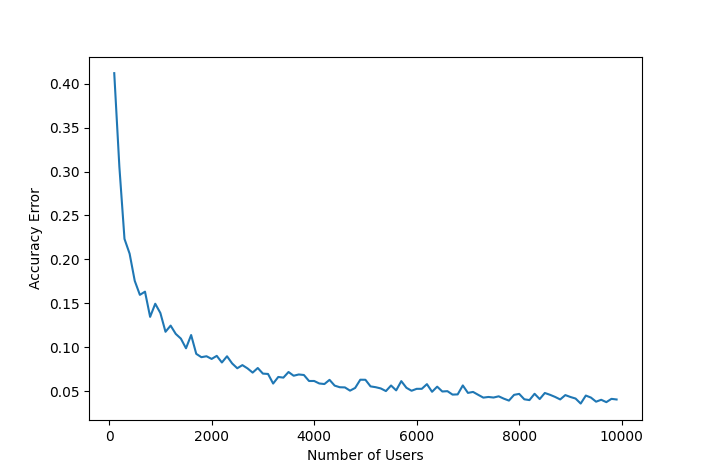
\includegraphics[width=0.8\textwidth]{images/rr_results.png}
    \caption{Accuracy Error in R.R for increasing values of epsilon}
\end{figure}


We observe that the plot behaves as expected: the protocol produces a logarithmic curve for the accuracy error, while for a large number of users(over 3000), the error stabilizes bellow $0.1$. 

\section{Simple Application of LDP}

The most simple of L.D.P. protocols is already mentioned in this Thesis, and is no other than the \textbf{Randomized Response} protocol. This algorithm implements the three steps mentioned in the introduction, as the user chooses a value (True or False), perturbs it(by the flipping of the coins), reports the perturbed value, with the sole job of the aggregator being to collect, normalize and report the values provided.


\section{Existing Protocols for Local DP}

Apart from R.R., many L.D.P. protocols have been implemented during the years, with many of them being widely used by companies in order to protect users' data. One of the most famous protocols is \textbf{RAPPOR}, created by Google, and being currently used in the Chrome browser in order for the company to provide useful info to its users without compromising their privacy. Also, Apple has created ts own protocol of L.D.P., and utilizes it in its products. 

However, we are not going to focus on those protocols moving forward, than the ones presented in [TODO: Insert cite], a paper which introduces many algorithms for L.D.P., each one with different perturbation techniques and suitable for different circumstances.

During this chapter we are going to give a definition of each algorithm, implement it using Python, and compare the accuracy results produced by those protocols, just like during our testings of the G.D.P. models. Each protocols has two parts: the \textbf{users} and the \textbf{aggregator}. For the users we must each time define the following functions:

\begin{itemize}
    \item $Encode()$: Encodes the true value that the user wants to report
    \item $Perturb()$: Perturbs the encoded value, in order to produce the random value that will be reported
\end{itemize}

For the aggregator we must each time define the  $Aggregate()$ function, that collects the reported random values of the users, and produces the results according to the model.

\subsection{Basic RAPPOR}
As mentioned earlier, RAPPOR is a protocol created by Google. Its simpler form, Basic RAPPOR is used in Chrome, where it collects answers to questions such as the user's home page. The protocol's functions are the following:

\textbf{Encoding:} $Encode(v) = A_0$, where $A_0$ is a d-bit vector, such that: $A_0[v] = 1$ and $A_0[i] = 1$ for every other i. 

\textbf{Perturbation:} The perturbation consists of 2 steps: the permanent and the instantaneous. The permanent one is carried out only one time, and is the following: $Perturb(A_0)$ = 



\chapter{CONCLUSIONS AND FUTURE WORK}
%   \lipsum[3-5]
  One reference to some paper \cite{manning:corenlp} and to another paper
  \cite{pennington:glove}.

\backmatter

% abbreviations table
\abbreviations
\begin{center}
	\renewcommand{\arraystretch}{1.5}
	\begin{longtable}{| l | @{\qquad} l |}
	\hline
	RDF    & Resource Description Framework \\
  \hline
	SPARQL & SPARQL Protocol and RDF Query Language \\
  \hline
	OWL    & Web Ontology Language \\
  \hline
	OGC    & Open Geospatial Consortium \\
	\hline
	\end{longtable}
\end{center}

% appendix
\begin{appendix}
% mark the beginning of the appendix
\appendixstartedtrue

% add appendix line to ToC
\phantomsection
\addcontentsline{toc}{chapter}{APPENDICES}

\chapter{FIRST APPENDIX}
\chapter{SECOND APPENDIX}
\chapter{THIRD APPENDIX}
\end{appendix}

% manually include the bibliography
\bibliographystyle{plain}
{\footnotesize \bibliography{references}}

% include it also in ToC (do sth on your own)
\addcontentsline{toc}{chapter}{REFERENCES}

\end{document}
